\documentclass[11pt,a4paper]{article}

% für \hyphenation mit Umlauten
\usepackage[T1]{fontenc}
\usepackage[utf8]{inputenc}
\usepackage[ngerman,english]{babel}

% Times-Roman-Schrift (auch für mathematische Formeln)
\usepackage{mathptmx} 

% comments
\usepackage{verbatim} 

% Zum Setzen von URLs
\usepackage{color}
\usepackage{alltt}
\definecolor{darkred}{rgb}{.25,0,0}
\definecolor{darkgreen}{rgb}{0,.2,0}
\definecolor{darkmagenta}{rgb}{.2,0,.2}
\definecolor{darkcyan}{rgb}{0,.15,.15}

\usepackage[plainpages=false,bookmarks=true,bookmarksopen=true,colorlinks=true,
  linkcolor=darkred,citecolor=darkgreen,filecolor=darkmagenta,
  menucolor=darkred,urlcolor=darkcyan]{hyperref}

% Zeilenabstand
\renewcommand{\baselinestretch}{1.5}

% anhang
\usepackage[toc,page]{appendix}

% pdflatex: Bilder in den Formaten .jpeg, .png und .pdf
% latex: Bilder im .eps-Format
\usepackage{graphicx}

\usepackage{fancyhdr} % Positionierung der Seitenzahlen
\fancyhead{}
\fancyfoot[C]{\Roman{page}}
\renewcommand{\headrulewidth}{0pt}
\setlength{\headheight}{13.6pt} % behebt headheight Warning

 % behebt headheight Warning
\setlength{\headheight}{13.6pt}

% Korrektes Format für Nummerierung von Abbildungen (figure) und
% Tabellen (table): <Kapitelnummer>.<Abbildungsnummer>
\makeatletter
\@addtoreset{figure}{section}
\renewcommand{\thefigure}{\thesection.\arabic{figure}}
\@addtoreset{table}{section}
\renewcommand{\thetable}{\thesection.\arabic{table}}
\makeatother

% Listings für Sourcecode
\usepackage{listings}
  \usepackage{courier}
 \lstset{
        basicstyle=\footnotesize\ttfamily, % Standardschrift
        numbers=left,               % Ort der Zeilennummern
        numberstyle=\tiny,          % Stil der Zeilennummern
        %stepnumber=2,               % Abstand zwischen den Zeilennummern
        numbersep=5pt,              % Abstand der Nummern zum Text
        tabsize=2,                  % Groesse von Tabs
        extendedchars=true,         %
        breaklines=true,            % Zeilen werden Umgebrochen
        keywordstyle=\color{red},
        frame=b,         
        keywordstyle=[1]{\color{DarkSkyBlue}},    % Stil der Keywords
        keywordstyle=[2]{\color{DarkScarletRed}},    %
        keywordstyle=[3]{\bfseries},    %
        keywordstyle=[4]{\color{DarkPlum}},    %
        keywordstyle=[5]{\color{SkyBlue}},    %
		stringstyle={\color{Chocolate}},
        showspaces=false,           % Leerzeichen anzeigen ?
        showtabs=false,             % Tabs anzeigen ?
        xleftmargin=17pt,
        framexleftmargin=17pt,
        framexrightmargin=5pt,
        framexbottommargin=4pt,
        backgroundcolor=\color{Aluminium1},
        showstringspaces=false,      % Leerzeichen in Strings anzeigen ?
		%language=php
		morekeywords=[1]{Interface,return,static,function}
}
    %\DeclareCaptionFont{blue}{\color{blue}} 

  %\captionsetup[lstlisting]{singlelinecheck=false, labelfont={blue}, textfont={blue}}
  \usepackage{caption}
\DeclareCaptionFont{white}{\color{white}}
\DeclareCaptionFormat{listing}{\colorbox[cmyk]{0.43, 0.35, 0.35,0.01}{\parbox{\textwidth}{\hspace{15pt}#1#2#3}}}
\captionsetup[lstlisting]{format=listing,labelfont=white,textfont=white, singlelinecheck=false, margin=0pt, font={bf,footnotesize}}
\renewcommand\lstlistingname{Codeblock}
 

\sloppy % Damit LaTeX nicht so viel über "overfull hbox" u.Ä. meckert

% Ränder
\addtolength{\topmargin}{-16mm}
\setlength{\oddsidemargin}{40mm}
\setlength{\evensidemargin}{40mm}
\addtolength{\oddsidemargin}{-1in}
\addtolength{\evensidemargin}{-1in}
\setlength{\textwidth}{13cm}
\addtolength{\textheight}{34mm}
%______________________________________________________________________

\hypersetup{
	pdfauthor = {Franziskus Domig, BSc;
		Stefan Gassner, BSc; Wolfgang Halbeisen,
		BSc; Matthias Schmid, BSc},
	pdftitle = {Projekt Dokumentation Roadrunner},
	pdfkeywords = {Roadrunner, Dokumentation, Transport, Logistik},
}

%======================================================================
%
%      Document
%
%======================================================================

\begin{document}

\selectlanguage{ngerman}

\pagestyle{empty} % Vorerst keine Seitenzahlen
\pagenumbering{alpha} % Unsichtbare alphabetische Nummerierung

\begin{center}
\textsc{Fachhochschule Vorarlberg GmbH}\\

\vspace{5cm}
{\large\textbf{Dokumentation}}\vspace{.5cm}

{\LARGE Roadrunner}

\end{center}

\vspace{14cm}


\begin{tabular}{ll}
Projektteam: & Franziskus Domig, Bsc; Stefan Gassner, BSc;\\
	     & Wolfgang Halbeisen, BSc; Matthias Schmid, BSc\\
Bearbeitung: & Dornbirn, im Sommersemester 2011\\
Betreuer:    & Prof.(FH) DI Wolfgang Auer\\
\end{tabular}

%______________________________________________________________________

\clearpage
\pagestyle{fancy}
\pagenumbering{roman} % Römische Seitenzahlen
\setcounter{page}{1}

\tableofcontents


\clearpage
\pagenumbering{arabic}
\setcounter{page}{1}
% Geändertes Format für Seitenränder, arabische Seitenzahlen
\fancyfoot[CO]{\thepage}

\input{input/preface}

\clearpage
\input{input/general}

\clearpage
\section{Technologie}
\label{sec:technology}

In diesem Abschnitt werden die von diesem Projekt verwendeten Technologien erläutert. Insbesondere werden die Gründe erläutert, weswegen diese Technologien eingesetzt und anderen vorgezogen werden.

\subsection{CouchDB}
\label{subsec:couchdb}
CouchDB\footnote{The Apache CouchDB Project, \url{http://couchdb.apache.org/}} ist eine auf die Verwaltung von Dokumenten basierte Datenbank. CouchDB kann ähnlich wie das MapReduce Framework von Google\footnote{vgl. \url{http://en.wikipedia.org/wiki/MapReduce}} abgefragt sowie indiziert werden.

TODO: Ausführlicher beschreiben.

\subsection{Node.js}
\label{subsec:nodejs}

Node.js ist ein ereignisgesteuertes I/O Framework für die V8 JavaScript Engine \cite{Wikipedia10a}. Node.js wurde in C++ sowie JavaScript entwickelt und liegt in einer MIT-Lizenz vor, welches es für dieses Projekt einsetzbar macht und zugleich auch in einem real logistischem Szenario eingesetzt werden könnte.

Der Vorteil von \textit{nodejs} liegt darin, dass sehr schnell, mit wenig
Zeilen Code und Aufwand ein Http-Server programmiert werden kann.

\subsection{Benötigte Packete}
\begin{itemize}
  \item nodejs (für Unix)
  \item npm (um Bilbliothek optimist komfortabel zu installieren)
  \item optimist (nodejs Library für Console-Parameter übergabe)
\end{itemize}


\subsection{Silex/PHP}

TODO

\subsection{Android/Java}

TODO

\subsection{Barscanner}

TODO

\clearpage
\input{input/database}

\clearpage
\section{CouchDB Applikation}
\label{sec:couchdb}

Apache CouchDB ist ein Dokument-Orientiertes-Datenbanksystem für die Verwendung
	mit JavaScript. CouchDB bietet inkrementelle Replikation mit bi-directionaler
	Konflikt-Erkennung und -Lösung.
	
CouchDB bietet eine REST-API \cite{Fowler10}[S. 1] via \emph{JavaScript Object
	Notation} (JSON) an, welche von jeder beliebigen Umgebung mit Hilfe von
	HTTP-Requests abgerufen werden kann. CouchDB ist zusätzlich ein System, welches
	eine beliebige Skalierbarkeit sowie Erweiterbarkeit anbietet
	\cite{CouchDB11}[S. 1].
	
In diesem Projekt wurde CouchDB eingesetzt, um ein relativ neues Gebiet der
	Datenpersistierung zu erlernen. Durch die einfache Replizierung von Daten,
	konnte CouchDB sowohl auf der Backend-Webapplikation (vgl.
	Kapitel~\ref{sec:webapplication}) als auch auf den mobilen Geräten (vgl.
	Kapitel~\ref{sec:android}) eingesetzt werden.

\subsection{Implementierung}

TODO: roadrunner.server

\subsubsection{JSON und Schema-Validierung}
Als Dokumentstruktur wird von CouchDB JSON verwendet. Vor der Speicherung eines
	JSON-Dokumentes in die Datenbank werden die Validierungsmethoden von allen
	Designdokumenten in der Datenbank aufgerufen. Nur wenn alle Validierungen
	erfolgreich sind wird das Dokument gespeichert. Obwohl JSON Schemalos ist
	kann trotzdem eine Schemavalidierung durchgeführt werden. Als Schema wird
	das JSON-Schema verwendet, dass sich aktuell in Version 03
	befindet \cite{IETF11}[S. 1]. 

In einem Designdokument können verschiedene Validierungen eingeführt werden.
	Zusätzlich zu Validierungen der Benutzerrechte werden in diesem Projekt alle
	Dokumente auf das definierte JSON-Schema validiert.

\subsubsection{Designdokumente}

TODO

\subsubsection{Dokumentänderung - MapReduce}

\emph{MapReduce} ist ein Framework von Google, dass entwickelt wurde damit sehr große
	Datenmengen parallel bearbeitet werden können. CouchDB verwendet ebenfalls
	einen ähnlichen Anstaz um Daten aus der Datenbank zu lesen. Anhand eines
	Beispieles wird die Funktionsweise von MapReduce nachfolgend erläutert.

Das Beispiel beantwortet folgende Problemstellung: Welche Gegenstände wurden
	von einer Transporteinheit (durch das Lesen des Barcodes) eingeladen
	und sind somit in der Datenbank als geladen gekennzeichnet?

\paragraph{Map - Phase} Auf jedes Dokument in der Datenbank wird die Map-Methode
	angewendet. In einer Map-Methode werden Key-Value-Paarungen gebildet. Jedes
	Dokument in der Datenbank kann eine beliebige Anzahl an Key-Value-Paarungen
	generieren. Diese Key-Value-Paarungen werden in einem B-Baum (vgl.
	\cite{Ottmann96}[S. 317-327]) gespeichert. Ändert sich nun ein Dokument müssen
	nur die entsprechenden Paarungen in	dem B-Baum angepasst werden. 

\paragraph{Reduce - Phase} In dieser Phase wird auf jeden Element in dem Baum die
	Reduce-Methode angewendet. Ziel der Reduce-Methode ist es die Datenmenge zu
	minimieren. Auf jedes Element kann die Reduce-Methode beliebig oft angewendet
	werden.

\subsection{Mögliche Erweiterungen}

TODO

\subsection{Verwendung in einem realen Projekt}

TODO

\clearpage
\section{Benutzergruppen}

Zur Umsetzung des Rechtesystems von Roadrunner werden verschiedene Benutzergruppen eingeführt. Die Rechte werden einerseits direkt auf der Datenbank definiert und zudem noch über Validierungsfunktionen umgesetzt. Die Benutzerauthentifizierung wird von CouchDB durchgeführt.

\subsection{Admins \& Readers}

\begin{figure}
	\centering
		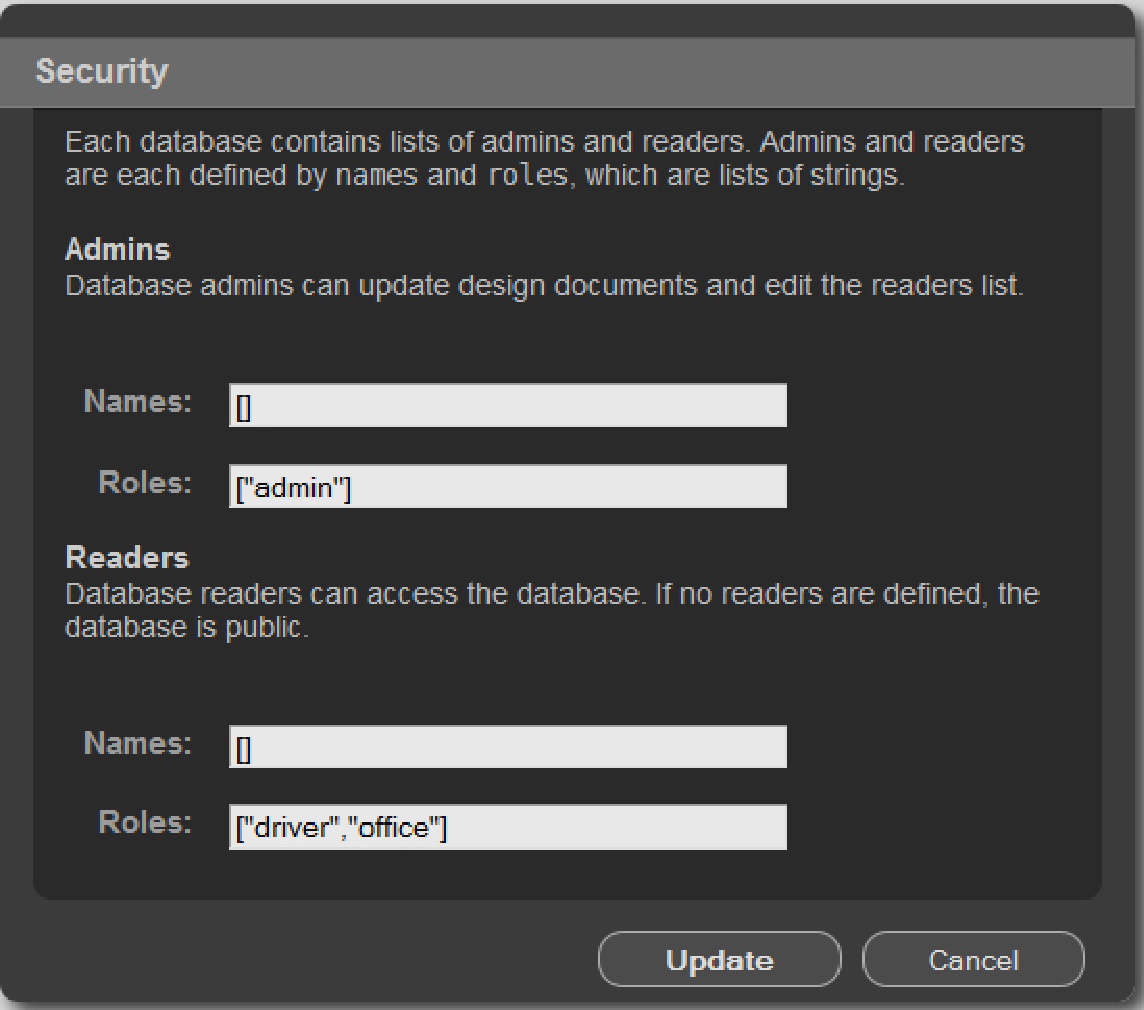
\includegraphics[width=0.8\textwidth]{files/pdf/security.pdf}
	\caption{Admins \& Readers}
	\label{fig:security}
\end{figure}

Auf einer Datenbank können in CouchDB Admins und Readers definiert werden. 
\begin{description}
\item[Admin] Ein Admin hat sämtliche Rechte auf der Datenbank. Er kann die zudem die Datenbank löschen, Designdokumente verändern oder Benutzerrechte ändern.
\item[Reader] Ein Reader hat lesenden und schreibenden Zugriff auf alle Dokumente bis auf die Designdokumente.
\end{description}

\noindent Ein Benutzer kann über 2 verschiedene Arten einer Gruppe zugeordnet werden:
 \begin{itemize}
\item Names: Ein CouchDB-Benutzer muss einen eindeutigen Namen im Format "`org.couchdb.user:[username]"' haben. Die Benutzer werden in einer seperaten Datenbank mit dem Namen "`\_users"' definiert. Wenn der Benutzer dieser Liste (Array aus Strings) hinzugefügt wird, dann besitzt er die entsprechenden Rechte.
\item Roles: Ein Benutzer kann verschiedene Rollen besitzen. Wenn eine seiner Rollen in dieser Liste aufgeführt wird, hat er die entsprechenden Rechte. 
\end{itemize}

\subsection{Rollen in Roadrunner}

Einem Benutzer können keine bis mehrere Rollen zugewiesen werden. Bei jeder Veränderung von Dokumenten auf dem Backendsystem wird von CouchDB eine Benutzerauthentifizierung durchgeführt. Bei dieser Benutzerauthentifizierung wird das Zugriffsrecht auf die Datenbank überprüft und zudem eine Validierung durchgeführt. Bei der Validierung werden alle definierten Validierungsmethoden aufgerufen. Nur wenn alle Validierungen gültig sind wird die gewünschte Änderung an den Dokumenten durchgeführt.
\newline \newline \noindent
Im Projekt Roadrunner wurden 3 verschiedenen Rollen definiert:
\begin{description}
\item[Admin] Ein Admin hat sämtliche Rechte auf der Datenbank. Diese Rollen ist ausschließlich für Administratoren vorgesehen.
\item[Office] Ein Benutzer der Gruppe Office arbeitet mit dem Backendsystem von Roadrunner. Dieser Benutzer arbeitet über die Webapplikation mit Roadrunner.
\item[Driver] Ein Benutzer der Gruppe Driver ist ein Fahrer. Er arbeitet auf dem Androidsystem mit Roadrunner. Auf dem Androidsystem arbeitet er als Admin mit der Datenbank. Eine Einschränkung der Benutzerrechte auf dem Androidsystem ist nicht nötig da die Benutzerauthentifizierung bei der Replizierung der Daten von dem Androidsystem auf das Backendsystem durchgeführt wird. Ein Fahrer kann nur Daten replizieren für die er die entsprechenden Rechte besitzt.
\end{description}

\noindent In den Validierungsmethoden werden die entpsrechenden Rechtevalidierungen durchgeführt. In Tabelle \ref{tab:rechte} sind die Berechtigungen aufgelistet. Ein + bedeutet, dass der Benutzer das Recht besitzt.

\begin{table}
\begin{tabular}{lccc}
& Driver & Office & Admin \\
Benutzerrechte ändern & - & - & + \\
Designdokumente ändern & - & - & + \\
Logeinträge anlegen & + & + & + \\
Logeinträge ändern & - & - & + \\
Logeinträge löschen & - & - & + \\
Andere Dokumente anlegen & - & + & + \\
Andere Dokumente ändern & - & + & + \\
Andere Dokumente löschen & - & + & +
\end{tabular}
\caption{Benutzerrechte}
\label{tab:rechte}
\end{table}

\clearpage
\section{Android}

\subsection{Voraussetzungen}

\subsection{Setup der Applikation}

\subsection{Komponenten}

Dieser Abschnitt beschreibt aus welchen Komponenten die Applikation besteht. Es gibt einen Service und eine Main-Activity.

\clearpage
\section{GIT}

\subsection{Unterschiede zu SVN}

\subsection{Arbeitsweise mit GIT}

\subsection{Mögliche Probleme}



\clearpage
\input{input/usecases}

\clearpage
\input{input/iteration1}

\clearpage
\section{Applikationssicherheit}

\subsection{Zeitsynchronisierung}

In diesem Abschnitt werden Probleme besprochen, die durch fehlerhafte respektive
mangelhaft durchdachte Zeitsynchronisierung oder Verbindungsabbruch entstehen
können.


\paragraph{Problem durch falsche Zeitstempel bei Logeinträgen:}
Betrachtet wird das Szenario ``Umladevorgang eines Produktes''. Das mobile
Gerät der Transporteinheit wird benutzt um den Ausladevorgang aus einem
Container im System zu verarbeiten. Mit dem scannen des Produkts wird auf dem
mobilen Gerät der Transporteinheit ein Logeintrag in dessen lokale Datenbank
erstellt. Genauso wird beim darauffolgenden Ladevorgang der Umladestation ein
Logeintrag auf dessen Gerät erstellt. Wenn das System mit absoluter Zeit
arbeitet und die Uhrzeit des Geräts der Transporteinheit vor jener der
Umladestation ist, dann würde im System der Übernahmevorgang der Umladestation
vor dem Ausladevorgang der Transporteinheit stattfinden.
\par
\paragraph{Lösungsansatz:}
Um dieses Problem zu lösen muss relative Zeit eingeführt und synchronisiert
werden. Für die Zeitsynchronisierung können bekannte Algorithmen für verteilte
Systeme eingeführt werden. Mögliche Algorithmen sind
\par

\paragraph{TODO:}
UPV distributed Clocks .. algorithmen herausfinden und oben einfügen\\ 

	Christian's Algorithm, Berkley Algorithm, 
	$http://en.wikipedia.org/wiki/Clock_synchronization$
\par

Grundsätzlich müssen diese Probleme berücksichtigt werden. In unserem
Projekt werden die erwähnten Lösungen aus zeitlichen Gründen und anderer
Zielsetzung nicht implementiert.

\subsection{Zugriffskontrolle}

Zur Umsetzung des Rechtesystems von Roadrunner werden verschiedene Benutzergruppen eingeführt. Die Rechte werden einerseits direkt auf der Datenbank definiert und zudem noch über Validierungsfunktionen umgesetzt. Die Benutzerauthentifizierung wird von CouchDB durchgeführt.

\subsection{Administratoren \& Benutzer}

\begin{figure}
	\centering
		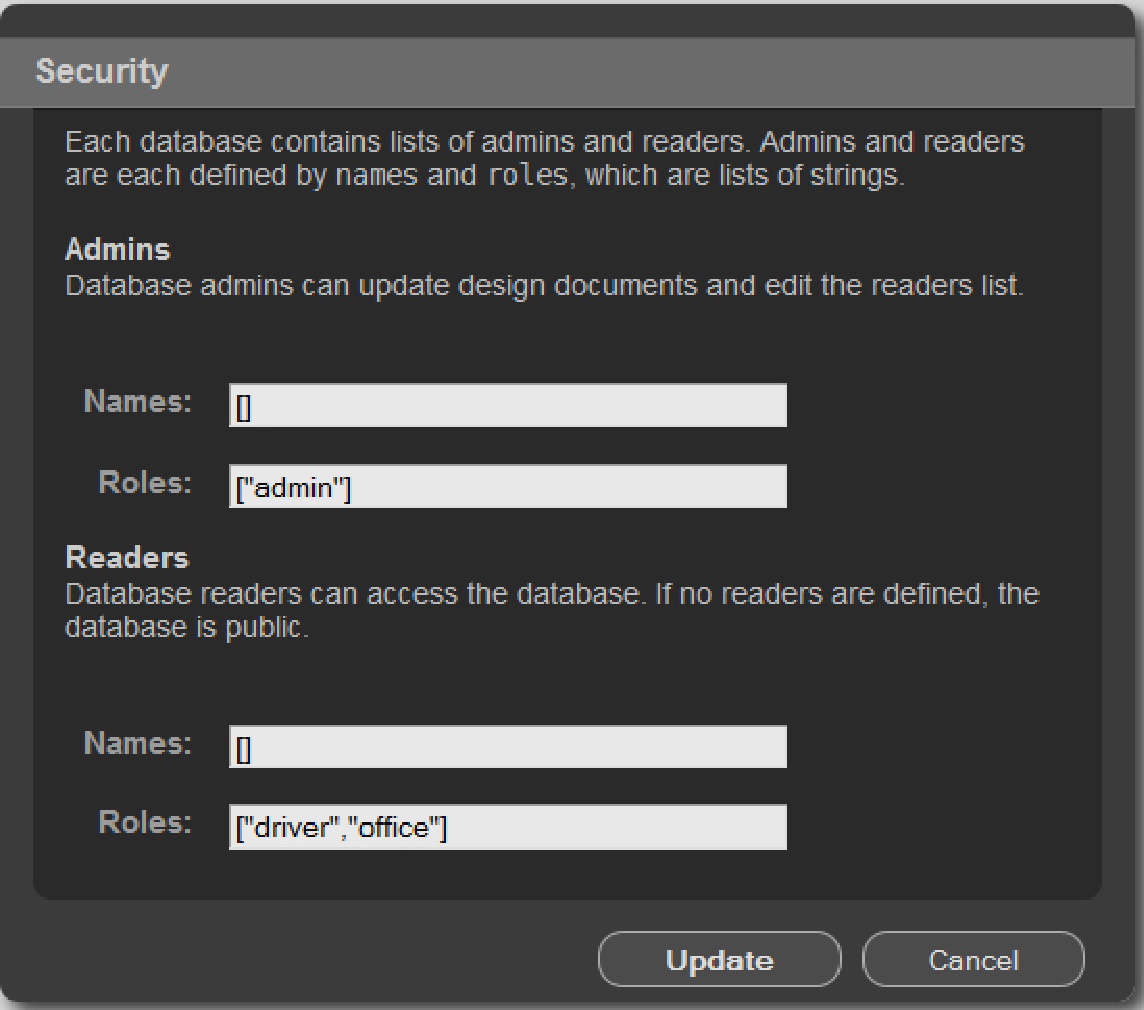
\includegraphics[width=0.8\textwidth]{files/pdf/security.pdf}
	\caption{Admins \& Readers}
	\label{fig:security}
\end{figure}

Auf einer Datenbank können in CouchDB Admins und Readers definiert werden. 
\begin{description}
\item[Admin] Ein Admin hat sämtliche Rechte auf der Datenbank. Er kann die zudem die Datenbank löschen, Designdokumente verändern oder Benutzerrechte ändern.
\item[Reader] Ein Reader hat lesenden und schreibenden Zugriff auf alle Dokumente bis auf die Designdokumente.
\end{description}

\noindent Ein Benutzer kann über 2 verschiedene Arten einer Gruppe zugeordnet werden:
 \begin{itemize}
\item Names: Ein CouchDB-Benutzer muss einen eindeutigen Namen im Format "`org.couchdb.user:[username]"' haben. Die Benutzer werden in einer seperaten Datenbank mit dem Namen "`\_users"' definiert. Wenn der Benutzer dieser Liste (Array aus Strings) hinzugefügt wird, dann besitzt er die entsprechenden Rechte.
\item Roles: Ein Benutzer kann verschiedene Rollen besitzen. Wenn eine seiner Rollen in dieser Liste aufgeführt wird, hat er die entsprechenden Rechte. 
\end{itemize}

\subsubsection{Rollen in Roadrunner}

Einem Benutzer können keine bis mehrere Rollen zugewiesen werden. Bei jeder Veränderung von Dokumenten auf dem Backendsystem wird von CouchDB eine Benutzerauthentifizierung durchgeführt. Bei dieser Benutzerauthentifizierung wird das Zugriffsrecht auf die Datenbank überprüft und zudem eine Validierung durchgeführt. Bei der Validierung werden alle definierten Validierungsmethoden aufgerufen. Nur wenn alle Validierungen gültig sind wird die gewünschte Änderung an den Dokumenten durchgeführt.
\newline \newline \noindent
Im Projekt Roadrunner wurden 3 verschiedenen Rollen definiert:
\begin{description}
\item[Admin] Ein Admin hat sämtliche Rechte auf der Datenbank. Diese Rollen ist ausschließlich für Administratoren vorgesehen.
\item[Office] Ein Benutzer der Gruppe Office arbeitet mit dem Backendsystem von Roadrunner. Dieser Benutzer arbeitet über die Webapplikation mit Roadrunner.
\item[Driver] Ein Benutzer der Gruppe Driver ist ein Fahrer. Er arbeitet auf dem Androidsystem mit Roadrunner. Auf dem Androidsystem arbeitet er als Admin mit der Datenbank. Eine Einschränkung der Benutzerrechte auf dem Androidsystem ist nicht nötig da die Benutzerauthentifizierung bei der Replizierung der Daten von dem Androidsystem auf das Backendsystem durchgeführt wird. Ein Fahrer kann nur Daten replizieren für die er die entsprechenden Rechte besitzt.
\end{description}

\noindent In den Validierungsmethoden werden die entpsrechenden Rechtevalidierungen durchgeführt. In Tabelle \ref{tab:rechte} sind die Berechtigungen aufgelistet. Ein + bedeutet, dass der Benutzer das Recht besitzt.

\begin{table}
\begin{tabular}{lccc}
	& Driver & Office & Admin \\
	Benutzerrechte ändern & - & - & + \\
	Designdokumente ändern & - & - & + \\
	Logeinträge anlegen & + & + & + \\
	Logeinträge ändern & - & - & + \\
	Logeinträge löschen & - & - & + \\
	Andere Dokumente anlegen & - & + & + \\
	Andere Dokumente ändern & - & + & + \\
	Andere Dokumente löschen & - & + & +
\end{tabular}
\caption{Benutzerrechte}
\label{tab:rechte}
\end{table}


\clearpage
\section{Transportüberwachung mittels Sensoren}\label{sensors}
\label{sec:sensors}

In diesem Projekt wurden die Transportüberwachung mittels Sensoren, welche
	von der Android Applikation (siehe Kapitel~\ref{sec:android})) überwacht
	werden, realisiert.
	
Für die in diesem Projekt spezifizierten Anforderungen (siehe Kapitel~\ref{sec:requirements})
	wurde die Temperatur sowie die aktuelle Position eines Gegenstands überwacht. Hierzu
	werden zwei unterschiedliche Sensortypen, welche in den beiden nachfolgenden Abschnitten
	erläutert werden, verwendet. Zusätzlich wurde die Zeitsynchronisation der mobilen Geräte
	mittels eigens entwickelter Synchronisierung (wie in Abschnitt~\ref{subsec:timesync}
	erläutert) realisiert.

\subsection{Temperaturüberwachung}

Temperatursensoren werden in diesem Projekt simuliert. Alle benötigten
	Temperatursensoren werden mit \emph{nodejs}, wie in
	Abschnitt~\ref{subsec:nodejs} erläutert, simuliert.

\subsection{Positionsüberwachung}

In diesem System werden in einem Zeitintervall von fünf Minuten die aktuelle
	Position eines auf dem Transportweg befinden Gegenstands aufgezeichnet.
	Die Positionsdaten werden von der Android Applikation bzw. der Service
	Applikation ausgelesen. Hierzu werden die Positionsdaten via GPS bzw. UMTS
	oder WLAN ermittelt und mit aufgezeichnet.
	
Die ermittelten Positionsdaten werden auf der Webapplikation bei den Lieferungen
	jeweils auf einer Karte dargestellt.


%______________________________________________________________________

\cleardoublepage
\pagenumbering{Roman}

\begin{thebibliography}{99}
\addcontentsline{toc}{section}{Literaturverzeichnis}

\bibitem[Gamma 94]{Gamma94}
  E.\ Gamma, R.\ Helm, R.\ Johnson, J.\ Vlissides:
    Design Patterns: Elements of Reusable Object-Oriented Software.
	MA: Addison-Wesley, 1994.

%    Web-References
%______________________________________________________________________

\hspace{-\leftmargin}{\Large\bfseries Web-Referenzen} % Wüster Hack %-|

\bibitem[Wikipedia 10a]{Wikipedia10a}
  Wikipedia: Node.js
    \url{http://de.wikipedia.org/wiki/Node.js}, besucht am 20.04.2011.

\end{thebibliography}


% ende des hauptteils
\fancyhead[R]{} % Keine Kopfzeile mehr oben auf jeder Seite

\end{document}
